\documentclass[a4paper,10pt]{article}
\usepackage{CJK}
\usepackage{indentfirst}
\usepackage{graphicx}
\usepackage{bibentry,natbib}
\usepackage{fancyhdr}
\usepackage{lastpage}

\usepackage[top=2.54cm, bottom=2.54cm, left=3.18cm, right=3.18cm]{geometry}
\begin{document}
\begin{CJK}{UTF8}{song}

\begin{center}
\Large OpenGL 光照模型
\end{center}
\section{光和材料}
对于光线来说,颜色成分的数量对应于每种颜色的完全强度的百分比。如果一种光线的颜色的R,G和B值都为1.0,这种光线就是可以实现的最亮白色。如果这些值都是0.5,这种光线应该是白色的,但强度只有一半,因些看上去像是灰色的。

对于材料而言,它的RGB的值和它对这些颜色的反射比例相对应,因些,如果一种材料的R=1,G=0.5,B=0,它将反射所有的入射红光,一半的入射绿光,但是不反射任何入射的蓝光。如果光线L的强度为(LR,LG,LB),材料M具有相应的成分为(MR,MG,MB),那么在忽略了其它所有的反效果之向,进入眼睛的光就是:
\begin{displaymath}
L\times{}M=(LR\times{}MR,LG\times{}MG,LB\times{}MB)
\end{displaymath}
如果在场景中有多个光源,那么进入眼睛的光为:
\begin{displaymath}
  \sum_{i=0}^{n}L_{i}\times{}M=\sum_{i=0}^{n}(LR_i\times{}MR,LG_i\times{}MG,LB_i\times{}MB)
\end{displaymath}

\section{法线与光照}
在OpenGL中,物体的法线向量决定了它相对于光源的方向。对于物体的每个顶点, OpenGL使用法线判断这个顶点从每个光源接收的光线数量。

\section{衰减因子}
在光线的传播过程中,光的强度可能会随着距离的增加而衰减,OpenGL支持三种衰减:常量衰减$k_{c}$,线性衰减$k_{i}$,二次衰减$k_{q}$。在光线传播距离为d时,衰减因子为:
\begin{displaymath}
  r=\frac{1}{k_{c}+k_{l}d+k_{q}d^{2}}
\end{displaymath}
衰减因子只对环境光,散射光和镜面光的强度都进行了衰减,但不对发射光和环境光的强度进行衰减。


\section{OpengGL的光照计算}
在启用光照之后,顶点颜色的计算公式如下:
\begin{displaymath}
  \begin{array}{ll} 
   \verb|顶点的颜色|=&\verb|顶点处的材料发射颜色| \\
		   &+\verb|全局环境光(在顶点处根据材料环境属性进行缩放)| \\
                   &+\verb|经过适当衰减的来自所有光源的环境、散射和镜面光成分|
  \end{array}
\end{displaymath}
在执行光照计算之后,颜色值将在[0,1]的范围之内(RGBA模式下)进行截取
\subsection{光源的贡献}
每个启用的光源都会对顶点的颜色做出贡献,这些贡献将会叠加在一起,公式为:
\begin{displaymath}
 \verb|每个光源的贡献=衰减因子|\times\verb|聚光灯效果|\times(\verb|环境光成分+散射光成分+镜面成分|)
\end{displaymath}
衰减因子的计算公式如下:
\begin{displaymath}
  \verb|衰减因子|=\frac{1}{k_{c}+k_{l}d+k_{q}d^{2}}
\end{displaymath}
其中: \\
\indent{}d=光源的位置和顶点之间的距离 \\
\indent{}$k_{c}$=常量衰减因子(GL\_CONSTANT\_ATTENUATION)   \\
\indent{}$k_{l}$=线性衰减因子(GL\_LINEAR\_ATTENUATION) \\
\indent{}$k_{q}$=二次衰减因子(GL\_QUADRATIC\_ATTENUATION) \\
\indent{}如果光源为线性光源,那么衰减因子为1

\subsection{聚光灯效果}
聚光灯效果根据是否为聚光灯以及顶点是否位于聚光灯的光锥范围之内取如下3个值之一:
\begin{itemize}
\item 如果光源不是聚光灯(GL\_SPOT\_CUTOFF为180.0),则取值为1;
\item 如果光源为聚光灯,但是顶点位于聚光灯的光锥的外面,则取值为0;
\item 其它情况为$max(v\cdot{}d,0)^{GL\_SPOT\_EXPONENT}$,其中:
\begin{enumerate}
 \item  $v=(v_x,v_y,v_z)$,它是从顶点指向聚光灯(GL\_POSTION)的单位向量;
 \item  $d=(d_x,d_y,d_z)$,它是聚光灯的方向(GL\_SPOT\_DIRECTION),它假定光源是聚光灯,并且顶点位于聚光灯所产生的光锥的内部
\end{enumerate}
v和d这两个向量的点积随新着它位之间角度的余弦值而发生改变。因些,正对聚光灯方向的物体能够得取最强的光照,离光锥轴线的位置越远,物体受到照射的强度也就越弱。
\end{itemize}

\subsection{环境光成分}
环境光成分就是光源的环境颜色根据村料的环境属性进行缩放后的值:
\begin{displaymath}
 ambient_{light}*ambient_{material}
\end{displaymath}

\subsection{散射光成分}
散射光成分需要考虑光线是否直接照射在顶点上,光源的散射颜色以及材料的散射属性:
\begin{displaymath}
 max(L\cdot{}n,0)*diffuse_{light}*diffuse_{material}
\end{displaymath}
其中:
\begin{enumerate}
 \item $L=(L_x,L_y,L_z)$,它是从顶点到光源位置(GL\_POSTION)的单位向量;
 \item $n=(n_x,n_y,n_z)$是顶点的单位法线向量;
\end{enumerate}

\subsection{镜面光成分}
镜面光成分取决于光线是否直接落在顶点上,如果$L\cdot{}n$小于等于0,顶点上就不存在镜面光。如果存在镜面光成分,它的值取决于如下因素:
\begin{itemize}
 \item 顶点$(n_x,n_y,n_z)$处的单位法线向量;
 \item 两个单位向量之和,这两个单位向量分别是:
  \begin{itemize}
    \item[a)] 从顶点指向光源位置(或光源方向)的向量;
    \item[b)] 从顶点指向观察点的向量(如果GL\_LIGHT\_MODEL\_LOCAL\_VIEWER为真),否则使用向量(0,0,1);
  \end{itemize}
把这两个向量的和规范化,产生s=$(s_x,s_y,s_z)$
\item 镜面指数(GL\_SHININESS);
\item 光源的镜面颜色(GL\_SPECULAR$_{light}$)
\item 材料的镜面属性(GL\_SPECULAR$_{material}$)
\end{itemize}
计算镜面成分的公式如下:
\begin{displaymath}
 max(s\cdot{}n,0)^{shininess}\times{}specular_{light}\times{}specular_{material}
\end{displaymath}

\subsection{完整的光照计算公式}
在RGBA模式下完整光照的计算公式如下:
\begin{displaymath}
\begin{array}{ll}
\verb|顶点颜色|= & emission_{meterial} \\
		&+ambient_{light\_mode}\times{}ambient_{material} \\
                &+\sum_{i=0}^{n-1}(\frac{1}{k_c+k_l\times{}d+k_q\times{}d^2})\times{}(\verb|聚光灯效果|)_i \\
		&\times{}[ambient_{light}\times{}ambient_{material}  \\
                &+max(L\cdot{}n,0)\times{}diffuse_{light}\times{}diffuse_{material}  \\
                &+max(s\cdot{}n,0)^{shininess}\times{}specular_{light}\times{}specular_{material} ]_i
\end{array}
\end{displaymath}

\subsection{镜面铺助颜色}
如果当前的光照模型颜色控制为GL\_SEPARATE\_SPECULAR\_COLOR,那么每个顶点都将产生主颜色和辅助颜色,它们的计算方法如下:
\begin{displaymath}
 \begin{array}{ll}
 \verb|主颜色|=&emission_{material}\\
	      &+ambient_{light\_mode} \times{} ambient_{meterial} \\
                &+\sum_{i=0}^{n-1}(\frac{1}{k_c+k_l\times{}d+k_q\times{}d^2})\times{}(\verb|聚光灯效果|)_i \\
		&\times{}[ambient_{light}\times{}ambient_{material}  \\
                &+max(L\cdot{}n,0)\times{}diffuse_{light}\times{}diffuse_{material}]_i
 \end{array}
\end{displaymath}
\begin{displaymath}
 \begin{array}{ll}
  \verb|辅助颜色|= &\sum_{i=0}^{n-1}(\frac{1}{k_c+k_l\times{}d+k_q\times{}d^2})\times{}(\verb|聚光灯效果|)_i \\
                &\times{}[max(s\cdot{}n,0)^{shininess}\times{}specular_{light}\times{}specular_{material} ]_i
 \end{array}\
\end{displaymath}
在进行纹理帖图时,只有主颜色与纹理颜色进行混合,在纹理操作之后,辅助颜色被添加到主颜色和纹理颜色混合所产生的颜色之中


\section{雾方程式}
雾根据雾的混合因子把雾颜色与源片断的颜色进行混合。这个因子f是根据下列3个方程式之一进行计算,并截取在[0,1]的范围之内
当FOG\_MODE为GL\_EXP时:
\begin{displaymath}
 f=e^{-(density\cdot{}z)}
\end{displaymath}
当FOG\_MODE为GL\_EXP2时:
\begin{displaymath}
 f=e^{-(density\cdot{}z)^2}
\end{displaymath}
当FOG\_MODE为GL\_LINEAR时:
\begin{displaymath}
 f=\frac{end-z}{end-start}
\end{displaymath}
不同参数值情况下雾浓度方程式如下图:
\begin{figure}[hbtp]
\centering
 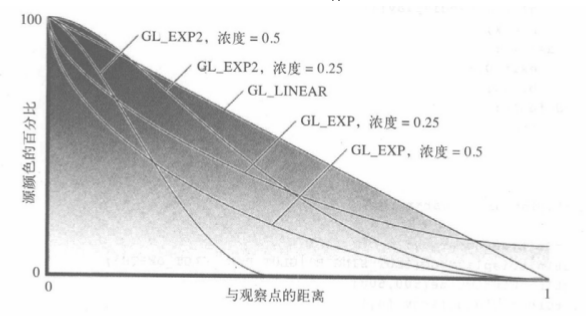
\includegraphics[height=60mm]{fog_dagram.png}
\end{figure}
在RGBA模式下,在启用雾的情况下,最终得到的颜色值为
\begin{displaymath}
 C=fC_{i}+(1-f)C_{f}
\end{displaymath}
其中$C_{i}$表示源片断的RGBA的值,$C_{f}$表示用\verb|GL_FOG_COLOR|分配的雾颜色值。








\end{CJK}
\end{document}




























